
\documentclass{article}
\usepackage[landscape]{geometry}
\usepackage{url}
\usepackage{multicol}
\usepackage{amsmath}
\usepackage{esint}
\usepackage{amsfonts}
\usepackage{tikz}
\usetikzlibrary{decorations.pathmorphing}
\usepackage{amsmath,amssymb}

\usepackage{colortbl}
\usepackage{xcolor}
\usepackage{mathtools}
\usepackage{amsmath,amssymb}
\usepackage{enumitem}
\makeatletter

\newcommand*\bigcdot{\mathpalette\bigcdot@{.5}}
\newcommand*\bigcdot@[2]{\mathbin{\vcenter{\hbox{\scalebox{#2}{$\m@th#1\bullet$}}}}}
\makeatother

\title{130 Cheat Sheet}
\usepackage[brazilian]{babel}
\usepackage[utf8]{inputenc}

\advance\topmargin-.8in
\advance\textheight3in
\advance\textwidth3in
\advance\oddsidemargin-1.5in
\advance\evensidemargin-1.5in
\parindent0pt
\parskip2pt
\newcommand{\hr}{\centerline{\rule{3.5in}{1pt}}}
%\colorbox[HTML]{e4e4e4}{\makebox[\textwidth-2\fboxsep][l]{texto}
\begin{document}

\begin{center}{\huge{\textbf{Modsim cheat sheet}}}\\
\end{center}
\begin{multicols*}{3}

\tikzstyle{mybox} = [draw=black, fill=white, very thick,
    rectangle, rounded corners, inner sep=10pt, inner ysep=10pt]
\tikzstyle{fancytitle} =[fill=black, text=white, font=\bfseries]

%------------ Simple rotations ---------------
\begin{tikzpicture}
\node [mybox] (box){%
    \begin{minipage}{0.3\textwidth}
        \begin{align*}
            R_x(\theta) =
            \begin{bmatrix}
                1 & 0 & 0 \\
                0 & \cos(\theta) & -\sin(\theta) \\
                0 & \sin(\theta) & \cos(\theta)
            \end{bmatrix}\\
            R_y(\theta) =
            \begin{bmatrix}
                \cos(\theta) & 0 & \sin(\theta) \\
                0 & 1 & 0 \\
                -\sin(\theta) & 0 & \cos(\theta)
            \end{bmatrix}\\
            R_z(\theta) =
            \begin{bmatrix}
                \cos(\theta) & -\sin(\theta) & 0 \\
                \sin(\theta) & \cos(\theta) & 0 \\
                0 & 0 & 1
            \end{bmatrix}
        \end{align*}
    \end{minipage}
};
%------------ Simple rotations header ---------------------
\node[fancytitle, right=10pt] at (box.north west) {Simple Rotations};
\end{tikzpicture}



%------------ Positive real ---------------
\begin{tikzpicture}
\node [mybox] (box){%
    \begin{minipage}{0.3\textwidth}
        $H(s)$ positive real iff
        \begin{enumerate}
            \item No poles with real part $> 0$
            \item $H(s)$ real for all positive and real s
            \item $\text{Re}[H(s)] \geq 0$ for all $\text{Re}[s] > 0$.
        \end{enumerate}
    \end{minipage}
};
\node[fancytitle, right=10pt] at (box.north west) {Positive Real};
\end{tikzpicture}


%------------ Eulers formula ---------------
\begin{tikzpicture}
\node [mybox] (box){%
    \begin{minipage}{0.3\textwidth}
        \begin{align*}
            e^{ix} = \cos(x) + i\sin(x)
        \end{align*}
    \end{minipage}
};
\node[fancytitle, right=10pt] at (box.north west) {Euler's Formula};
\end{tikzpicture}



%------------ Hyperbolic trig ---------------
\begin{tikzpicture}
\node [mybox] (box){%
    \begin{minipage}{0.3\textwidth}
        \begin{align*}
            \sinh(\sigma + j \omega) = \sinh \sigma \cos \omega + j \cosh \sigma \sin \omega \\
            \cosh(\sigma + j \omega) = \cosh \sigma \cos \omega + j \sinh \sigma \sin \omega \\
        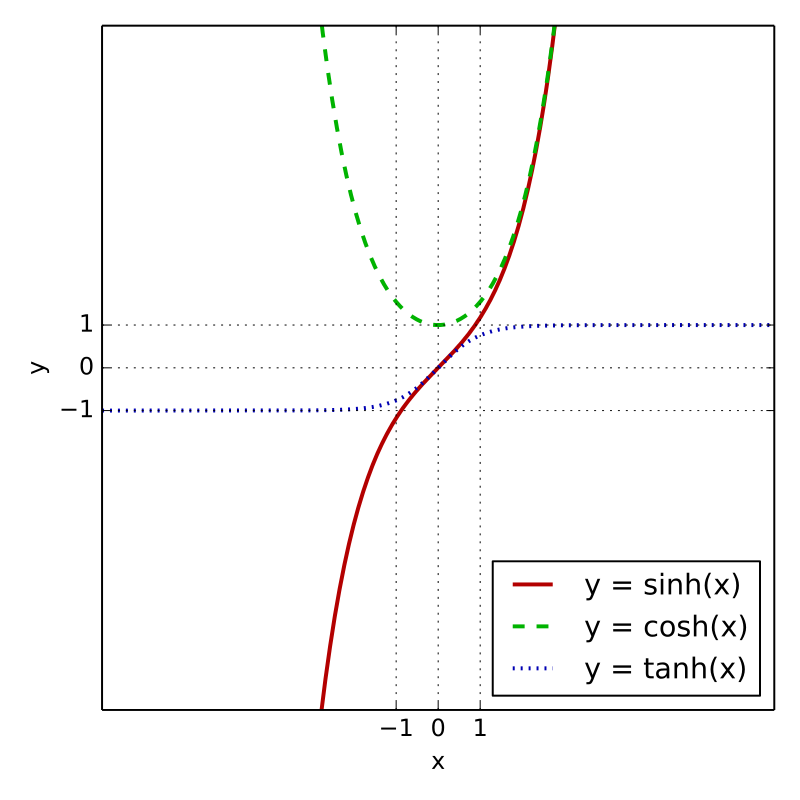
\includegraphics[width=0.5\textwidth]{hyp.png}
        \end{align*}
    \end{minipage}
};
\node[fancytitle, right=10pt] at (box.north west) {Hyperbolic Trig};
\end{tikzpicture}


%------------ Skew symmetric matrix ---------------
\begin{tikzpicture}
\node [mybox] (box){%
    \begin{minipage}{0.3\textwidth}
        \begin{align*}
            \mathbf{a} = \begin{bmatrix}
                a_1 \\
                a_2 \\
                a_3 
            \end{bmatrix}
            \iff
            \mathbf{a}^\times = \begin{bmatrix}
                0 & -a_3 & a_2 \\
                a_3 & 0 & -a_1 \\
                -a_2 & a_1 & 0
            \end{bmatrix}
        \end{align*}
        \begin{itemize}
            \item $u \times v$ corresponds to $\mathbf{u}^\times \mathbf{v}$
            \item $(\mathbf a^\times)^\top = -(\mathbf a^\times)$
        \end{itemize}
    \end{minipage}
};
\node[fancytitle, right=10pt] at (box.north west) {Skew Symmetric Matrix};
\end{tikzpicture}

\end{multicols*}
\end{document}

